\documentclass[11pt, letterpaper]{article}
\usepackage[top=1in, bottom=1in, left=1in, right=1in]{geometry}

% Math, graphics, and bibliography
\usepackage{amsmath,amssymb,amsfonts,mathrsfs,mathtools}

% My preferred fonts
\usepackage[T1]{fontenc}
\usepackage{lmodern}
\usepackage[sc]{mathpazo}
\usepackage{textcomp}

\usepackage{color}
\usepackage{tcolorbox}
\tcbuselibrary{breakable}
\tcbuselibrary{skins}
\usepackage{units}

\usepackage[parfill]{parskip} % For block paragraphs
\definecolor{gray}{gray}{0.4}
\newenvironment{reviewer}{\itshape\color{gray}}{}

\tcbset{skin=enhanced}

\newenvironment{manuscript}[1]{\begin{center}\begin{tcolorbox}[colback=green!5!white,colframe=green!75!black,width=0.8\textwidth,title={#1},breakable,fonttitle=\bfseries]}{\end{tcolorbox}\end{center}}


\begin{document}
\today\\

{\itshape Francis J. Doyle III}\\
Dept.\ of Chemical Engineering\\
Univ.\ of California, Santa Barbara\\
Santa Barbara, CA 93106-5080\\

{\itshape Leah Edelstein-Keshet}\\
Editorial Board Member\\
Biophysical Journal\\

Thank you for your email on September 24th, 2014, inviting us to submit a revised version of our manuscript, ``Amplitude metrics for cellular circadian bioluminescence reporters'' (MS: 2014BIOPHYSJ304278R) by Peter C. St. John, Stephanie R. Taylor, John H. Abel, and Francis J. Doyle~III.

We thank the reviewers for their second round of comments on the manuscript, in particular Reviewer \#2 for their continued attention to detail. We believe addressing these remaining concerns and suggestions have greatly improved the manuscript.

Please see our detailed responses to the reviewers below: 

\section*{Reviewer \#1}
\begin{reviewer}
The authors have largely responded you my concerns. 
 
Typos and suggestions 
 
- p. 2: "fail to capture the collective dynamics of a population oscillators" 
\end{reviewer}

This typo has been addressed, and the sentence now reads:

\begin{manuscript}{Page 2}
  Ordinary differential equation (ODE) models of gene regulation are capable of describing the amplitude and phase-resetting behavior of single cells, but fail to capture the collective dynamics of a population {\bfseries of} oscillators.
\end{manuscript}
 
\begin{reviewer}
- mu is defined a few lines after it is first used in Eq. (20). Perhaps define it first? 
\end{reviewer}

This change has also been made.

\begin{manuscript}{Page 7}
To define an amplitude change metric for such a case, we compare a perturbed trajectory $x(t)$ to a phase-shifted limit cycle reference $y(t)$, for which $x(t) \to y(t)$ for sufficiently long times.
Since $x(t)$ approaches the reference as $t \to \infty$, {\bfseries the means of both trajectories are equal and can be calculated by
\begin{equation}
  \mu \coloneqq \int_0^{2\pi} \frac{x^\gamma(\theta)}{2\pi} \; d\theta.
  \tag{20}
\end{equation}
The amplitude change metric is defined as}
\begin{equation}
  \begin{aligned}
    \Delta A (x(t), y(t)) &\coloneqq \int_0^\infty (x(t) - \mu)^2 - (y(t) - \mu)^2 \; dt\\
    &= \int_0^\infty h(t) \; dt.
  \end{aligned}
  \tag{21}
\end{equation}
\end{manuscript}

\section*{Reviewer \#2}
\begin{reviewer}
The revised manuscript becomes much more clear. The authors addressed most of my concerns in their revision. However, I have still couple concerns regarding the manuscript. 
 
1) In the previous review, I was concerned about using the Gillesplie algorithm for the model with non-elementary reactions because recent studies have clearly showed the inaccuracy of doing that (Thomas, Straube and Grima BMC Syst Biol (2012), Agarwal et al. J Chem Phy (2012) and Kim, Josic and Bennett Biophy J (2014)). Regarding this concern, the author showed that their continuous approximation also works for the model based on mass-action kinetics (Model 2). But, in the manuscript, the approximation is more accurate for Model 2 than other models, which are based on non-elementary reactions. This indicates that the inaccuracy coming from the Gillespie algorithm with non-elementary reaction appears to contribute the error seen in Model 1 and 3. Furthermore, I am mostly concerned that this manuscript can mislead the audience that using Gillespie algorithm with non-elementary reactions is justified. Please, clearly discuss the limitation in this approach. 
\end{reviewer}

This is a fair criticism, as we did not intend to defend the use of the stochastic simulation algorithm for non-elementary propensity functions. 
However, we believe the use of the algorithm in this case is justified, and is not the main source of error in the continuous approximation.
We provide a more detailed defense of our use of the algorithm for the reviewer's specific concerns below, and have incorporated additional disclaimers in the text to warn readers against the use non-elementary propensity functions in the general case.

There has indeed been a great deal of literature concerning the accuracy of using the Gillespie stochastic simulation algorithm for non-elementary propensity functions.
In K. R. Sanft, {\itshape et al, IET Syst. Biol.} (2011), the authors conclude that the Michealis-Menten approximation overestimates the noise of the corresponding full system of equations.
In L. A. Widmer, {\itshape et al, J. Chem. Phys.} (2013), the authors prove that the noise of the full system is bounded on $[\nicefrac{3}{4}, 1]$ of the noise estimated by the Michealis-Menten approximation.
For Hill-type kinetics, the full system can take an arbitrary level of noise relative to the approximated system (L. A. Widmer, Master's Thesis, 2013).

The most important consideration is that converting the models to a full mass-action description of the system (or to a slightly less detailed total quasi-steady-state approximation as discussed in the literature cited by the reviewer) would require additional parameter values to be chosen.
This parameter set is not identifiable, as an infinite number of parameter choices exist that will yield equivalent continuous dynamics to the Hill approximation.
Each of these parameter sets will have different noise characteristics, which may not be reflected by the arbitrary noise characteristics arising from the Hill simplification.
However, since we do not specify these expanded parameters, we simply fit the noise characteristics of the approximated model (using the volume parameter) to yield physiologically realistic desynchronization rates.
Therefore, the validity of whether or not these approximated solutions closely represent the noise characteristics of the full solutions does not play a large role in determining the accuracy of the continuous approximation.

To address the larger point, we discuss reasons why our continuous approximations are less accurate for the larger model than the smaller model. 
We first point out that the method is an asymptotic approximation of a population of oscillators in the limit of no noise, as we account for the noise-induced desynchronization of oscillators but not noise-induced deviation from the limit cycle.
When noise is present, the `unperturbed' population consists of oscillators not only with a distribution of phases, but also with the states of each oscillator in a region of space near the deterministic limit cycle (this can be seen in the left plot of supplemental movies S1 \& S2).
As a result, the responses of oscillators not directly on the limit cycle to a pulse can differ from their limit cycle counterparts, decreasing the accuracy of the method for systems with high noise.
In practice, however, it takes a considerable amount of noise before the continuous predictions deviate substantially from the stochastic populations.
It is also important to consider that the larger model consists of many more state variables than the mass-action model, only one of which is shown in Fig.~S3.
Therefore, the difference in accuracy likely comes from increased deviation about the deterministic limit cycle in 8 spatial dimensions, rather than from non-elementary propensity functions.

We have endeavored to make these points more clear in the manuscript:

\begin{manuscript}{Supplemental Info, Page 6}
Good agreement is seen between the continuous and stochastic simulations, indicating the proposed method is suitable for predicting the population-level responses for a variety of model types.
{\bfseries The slightly reduced accuracy seen in the larger Model 2 demonstrates a limitation of the method, which should be considered before applying the method to extreme cases.
As Eq.~44 tabulates the response of the system from the limit cycle, systems which are perturbed from states far from the deterministic limit cycle will not be captured appropriately.
Therefore, the difference in accuracy between Model 2 and Model 3 likely comes from increased deviation about the deterministic limit cycle in a greater number of spatial dimensions.}
\end{manuscript}

Additionally, we caution readers against the unchecked use of the Gillespie algorithm for systems with non-elementary propensity functions:

\begin{manuscript}{Supplemental Info, Page 6}
{\bfseries Model 1:}
Adapted from Nov\'{a}k \& Tyson, 2008 (1). Model used for
ARC demonstrations in Figs. 1-3, S1 ($P=4$) and Fig. S2, Movies S1 \& S2
($P=2$).
{\bfseries It should be noted that the use of the stochastic simulation algorithm for reactions with non-elementary propensities may inaccurately represent the noise of the full system.
In this case, we simply fit the noise characteristics of the approximated model (using the volume parameter) to yield physiologically realistic desynchronization rates. The volume of the stochastic simulations was chosen as $\Omega = 250$.}
\end{manuscript}

\begin{reviewer}
2) Another concern is regarding the major result of the manuscript (Fig. 5). The author perturbed the degradation of Per mRNA parameter in response to light. However, this conflicts with the previous experimental studies, which have shown that light promotes the transcription of Per mRNA via CREB, not degradation. 
\end{reviewer}

This is a valid point, since our analysis captures the increase in {\itshape Per} mRNA following light pulses as a {\itshape\bfseries decrease} in the degradation rate of {\itshape Per}.
In the model, {\itshape Per} transcription is controlled by several parameters: the maximum transcription rate, transcription rate kinetic constant, maximum degradation rate, degradation rate kinetic constant, and translation rate.
Since we acknowledge that the model does not perfectly describe the true system, we tried to fit the model to data by searching the parameter ARCs for parameters and reporter states which gave the appropriate response. 
From these parameters, the maximum {\itshape Per} transcription rate and {\itshape Cry} mRNA emerged as the best choice given the response of the model and known experimental results. We have added the following text to the manuscript to make this point more apparent:

\begin{manuscript}{Page 16}
The next step in capturing the experimental data was finding a perturbation capable of desynchronizing the system.
To find such a perturbation, we calculated population-level ARCs at several different knockdown strengths for each parameter in the model.
We selected the degradation rate of {\itshape Per} mRNA from the feasible parameters due to PER's known induction by CREB following photo-perturbation (46). 
{\bfseries While not an exact match of the experimental system, reducing degradation rate yields a similar response to increasing transcription.}
The parameter was reduced by $28.5\%$ during the light pulses, a value fit to maximize light-induced desynchrony.
The output variable, PER2-luciferase in the experimental system, was chosen to be represented by {\itshape Cry1} mRNA - an E box activated gene that is buffered from the direct effects of the parameter perturbation.
\end{manuscript}

We should emphasize that we are not predicting {\itshape Per} induction following light actually occurs via degradation, but rather that by acknowledging the model does not perfectly capture the experimental system, we simply seek a qualitatively accurate description of the underlying phenomena.

\begin{reviewer}
3) The key goal of this manuscript is distinguishing the single-cell level and population-level amplitude change. For this, the authors applied their tool to the experimental data (Fig. 5). However, Fig. 5 does not clearly show how their tool achieves such goal. Please provide additional figures. For instance, $x_{ss}$ (steady-state perturbed trajectory) for perturbed and unperturbed cases, $p(\theta, t)$ for unperturbed case as well as perturbed case etc, so that readers can clearly see the difference of effect via single cell level and population level.  
\end{reviewer}

This is a good suggestion, and we thank the reviewer for helping us clarify our results.
We have added a figure to explicitly highlight the contributions from the population and single-cell level.
Due to lack of space in the main text and desire not to further complicate the original figure, we have added this figure as Figure~S4.
A reference to the figure was added to the main text of the manuscript:

\begin{manuscript}{Page 16}
The phase probability density function for the light-sensitive model trajectory is shown in Fig.~5C for several representative time points.
\ldots
{\bfseries Amplitude change in this case is mediated both at the population and single-cell level, as indicated by their representative ARCs. The contributions from each source are summarized in Fig.~S4.}
\end{manuscript}

with the following figure and caption added to the supplementary material:

\begin{manuscript}{Supplemental Info, Page 7}
  \begin{center}
    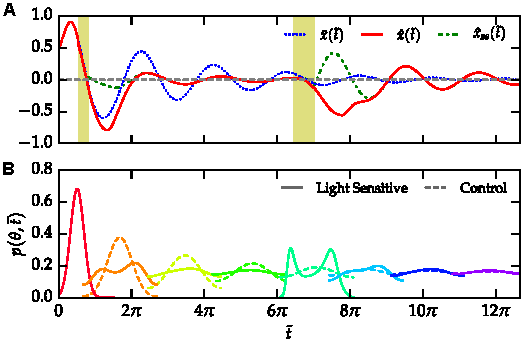
\includegraphics[width=.85\textwidth]{figures/figure_S4.pdf}\\
  \end{center}
{\bfseries Figure S4: Evidence of single-cell and population-level amplitude change.}
({\bfseries A}) The simulated control trajectory as shown in Fig.~5 is plotted again as $\bar{x}(\tilde{t})$.
The simulated light-sensitive trajector is also replotted as $\hat{x}(\tilde{t})$, which incorperates both single-cell and population-level effects.
The difference between this trajectory and the steady-state perturbed trajectory following both pulses, $\hat{x}_{ss}(\tilde{t})$, demonstrates the effect of single-cell level amplitude change in this particular case. 
Single-cell amplitudes are greatly increased following the first pulse, and altered significantly following the second.
({\bfseries B})
Comparison of the population densities for the control (dashed) and perturbed (solid) simulations.
The perturbed population is greatly desynchronized following the first light pulse, as indicated by its flatness relative to the control population. 
Following the second pulse, the perturbed population is more concentrated than the control, indicating higher amplitudes. 
These comparisons demonstrate the changes in population synchrony which occur due to the light pulse. 
\end{manuscript}

We would like to once again thank all our reviewers, as we feel our manuscript has benefited greatly from their suggestions and critiques.

\end{document}
